%This is a very basic  BE PROJECT PRELIMINARY template.

%############################################# 
%#########Author :  PROJECT###########
%#########COMPUTER ENGINEERING############


\documentclass[oneside,a4paper,12pt]{report}
%\usepackage{showframe}
%\hoffset = 8.9436619718309859154929577464789pt
%\voffset = 13.028169014084507042253521126761pt

\fancypagestyle{plain}{%
  \fancyhf{}
  \fancyfoot[CE]{AVCOE, Sangamner, Department of Computer Engineering 2023-24}
  \fancyfoot[RE]{\thepage}
}
\pagestyle{fancy}
\fancyhead{}
\renewcommand{\headrulewidth}{0pt}
\footskip = 0.625in
\cfoot{}
\rfoot{}

\usepackage[]{hyperref}
\usepackage{tikz}
\usetikzlibrary{arrows,shapes,snakes,automata,backgrounds,petri}

\usepackage{tabularx}
\usepackage[nottoc]{tocbibind}
%\usepackage[nottoc,notlot,notlof,numbib]{tocbibind}
\usepackage[titletoc]{appendix}
\usepackage{titletoc}
\renewcommand{\appendixname}{Annexure}
\renewcommand{\bibname}{References}

\setcounter{secnumdepth}{5}

\usepackage{float}
\usepackage{subcaption}
\usepackage{multirow}

\usepackage[ruled,vlined]{algorithm2e}

\begin{document}

\setlength{\parindent}{0mm}
\begin{center}
{\bfseries SAVITRIBAI PHULE PUNE UNIVERSITY \\}
 \vspace*{1\baselineskip}
{\bfseries A PROJECT REPORT ON \\}
 \vspace*{1\baselineskip}
{\bfseries \fontsize{16}{12} \selectfont PROJECT TITLE \\ \vspace*{2\baselineskip}}
{\fontsize{12}{12} \selectfont SUBMITTED TO THE SAVITRIBAI PHULE PUNE UNIVERSITY, PUNE
IN THE PARTIAL FULFILLMENT OF THE REQUIREMENTS 
FOR THE AWARD OF THE DEGREE \\
\vspace*{2\baselineskip}}
{\bfseries \fontsize{14}{12} \selectfont 
\hspace{18 mm}BACHELOR OF ENGINEERING
\newline(Computer Engineering) \\
\vspace*{1\baselineskip}} 
{\bfseries \fontsize{14}{12} \selectfont SUBMITTED BY \\ 
} 
\begin{center}
\bf{Group ID : AXX}
\end{center}
Student Name  \hspace{25 mm} Exam No:  \\
Student Name \hspace{25 mm} Exam No:   \\
Student Name \hspace{25 mm} Exam No:  \\
Student Name \hspace{25 mm} Exam No:\\
\vspace*{1\baselineskip}
{\bfseries \fontsize{14}{12} \selectfont Under The Guidance of \\  
\vspace*{1\baselineskip}} 
\bf{Prof. Guide Name}\\

\includegraphics[width=100pt]{AVCOE_LOGO.png} \\
{\bfseries \fontsize{14}{12} \selectfont DEPARTMENT OF COMPUTER ENGINEERING \\
Amrutvahini College of Engineering, Sangamner\\
Amrutnagar, Ghulewadi - 422608 \\
2023-24
}
\end{center}

\newpage

\begin{figure}[ht]
\centering

\includegraphics[width=100pt]{AVCOE_LOGO.png}
\end{figure}


{\bfseries \fontsize{14}{12} \selectfont \centerline{AMRUTVAHINI COLLEGE OF ENGINEERING,SANGAMNER}
\centerline{DEPARTMENT OF COMPUTER ENGINEERING}
\vspace*{1\baselineskip}} 


{\bfseries \fontsize{16}{12} \selectfont \centerline{CERTIFICATE} 
\vspace*{1\baselineskip}} 

\centerline{This is to certify that the Project Entitled}
\vspace*{1\baselineskip} 


{\bfseries \fontsize{14}{12} \selectfont \centerline{PROJECT TITLE}
\vspace*{1\baselineskip}}

\centerline{Submitted by}
\vspace*{1\baselineskip}
\centerline{\bf{Group ID: AXX}}  
\centerline{Student Name  \hspace{25 mm} Exam No: } 
\centerline{Student Name \hspace{25 mm} Exam No:  } 
\centerline{Student Name \hspace{25 mm} Exam No: }
\centerline{Student Name \hspace{25 mm} Exam No: }
\vspace*{1\baselineskip} 
are bonafide students of this institute and the work has been carried out by them under the supervision of  Prof. A. B. C and it is approved for the partial fulfillment of the requirement of Savitribai Phule Pune University, for the award of the degree of Bachelor of Engineering (Computer Engineering). \\\\
\bgroup
\def\arraystretch{0.7}
\begin{tabular}{c c }
Prof. Guide Name &  \hspace{50 mm} Dr. R. G. Tambe Dr. D. R. Patil \\								
Internal Guide   &  \hspace{50 mm} Project Coordinator \\
Dept. of Computer Engg.  &	\hspace{50 mm}Dept. of Computer Engg.  \\
\end{tabular}
 \vspace*{1.5\baselineskip}                     
                                                   
\begin{tabular}{c c }
Dr. S. K. Sonkar &  \hspace{50 mm} Dr. M.A. Venkatesh \\								
H.O.D.   &  \hspace{50 mm} Principal \\
Dept. of Computer Engg.  &	\hspace{50 mm}AVCOE Sangamner  \\
\end{tabular}
%}


\newpage

\begin{center}
{\bfseries SAVITRIBAI PHULE PUNE UNIVERSITY \\}
\end{center}

\begin{figure}[ht]
\centering

\includegraphics[width=150pt]{sppu_logo.jpg}
\end{figure}

{\bfseries \fontsize{16}{12} \selectfont \centerline{CERTIFICATE} 
\vspace*{1\baselineskip}} 

\centerline{This is to certify that,}
\vspace*{1\baselineskip} 
\vspace*{1\baselineskip}
\centerline{\bf{Group ID: AXX}}  
\centerline{Student Name  \hspace{25 mm} Exam No: } 
\centerline{Student Name \hspace{25 mm} Exam No:  } 
\centerline{Student Name \hspace{25 mm} Exam No: }
\centerline{Student Name \hspace{25 mm} Exam No: }

\centerline{of BE Computer Engineering was examined in the Project Examination entitled}
\vspace*{1\baselineskip}}

{\bfseries \fontsize{14}{12} \selectfont \centerline{PROJECT TITLE}
\vspace*{1\baselineskip}}

\centerline{on    \hspace{5 mm} /  \hspace{5 mm} / 2024}

\centerline{At}
\vspace{5 mm}

\centerline{DEPARTMENT OF COMPUTER ENGINEERING}
\centerline{AMRUTVAHINI COLLEGE OF ENGINEERING, SANGAMNER}
 
\vspace{10 mm}
\def\arraystretch{0.7}
\begin{tabular}{c c }
 &  \hspace{50 mm} \\						
\line(1,0){90}   &  \hspace{60 mm}\line(1,0){90} \\
Internal Examiner   &  \hspace{60 mm} External Examiner \\
\end{tabular}
 \vspace*{1.5\baselineskip}                     
                                                   


\newpage

%\pictcertificate{TITLE OF BE PROJECT}{Student Name}{Exam Seat No}{Guide Name}
\setcounter{page}{0}
\frontmatter
\cfoot{AVCOE, Department of Computer Engineering 2023-24}
\rfoot{\thepage}
\pagenumbering{Roman}
%\pictack{BE PROJECT TITLE}{Guide Name}



\addcontentsline{toc}{chapter}{Acknowledgment}
\newpage
{\fontsize{16}{15} \bfseries \LARGE \selectfont \centerline{Acknowledgment}}
%{  \newpage {\bfseries \fontsize{14}{12} \selectfont \centerline{Acknowledgment} 
%\vspace*{2\baselineskip}} \setlength{\parindent}{11mm} }
%{ \setlength{\parindent}{0mm} }
\vspace{10mm}

Please Write here Acknowledgement. 

\addcontentsline{toc}{chapter}{Abstract}
\newpage
{\fontsize{16}{15} \bfseries \LARGE \selectfont \centerline{Abstract}}
%{  \newpage {\bfseries \fontsize{14}{12} \selectfont \centerline{Abstract} 
%\vspace*{2\baselineskip}} \setlength{\parindent}{11mm} }
%{ \setlength{\parindent}{0mm} }
\vspace{10mm}

Please Write here Abstract.It should mainly include introduction, motivation,outcome and innovation if any.\\

\addcontentsline{toc}{chapter}{Synopsis}
\newpage
{\fontsize{16}{15} \bfseries \LARGE \selectfont \centerline{Synopsis}}
%{\newpage {\bfseries \fontsize{14}{12} \selectfont \centerline{Synopsis} 
%\vspace*{2\baselineskip}} \setlength{\parindent}{11mm} }
%{ \setlength{\parindent}{0mm} }
\vspace{10mm}

Add synopsis which was finalised at the start of Semester. 

\addcontentsline{toc}{chapter}{Abbreviation}
\newpage
{\fontsize{16}{15} \bfseries \LARGE \selectfont \centerline{Abbreviation}}
%{  \newpage {\bfseries \fontsize{14}{12} \selectfont \centerline{Acknowledgment} 
%\vspace*{2\baselineskip}} \setlength{\parindent}{11mm} }
%{ \setlength{\parindent}{0mm} }
\vspace{10mm}

\begin{tabular}{ll}
EM & Electomagnetic\\ 
EMS & Electomagnetic spectrum\\ 
MS & Multispectral\\
HS& Hyperspectral\\
LiDAR&  Light Detection and Ranging\\
\end{tabular}

\addcontentsline{toc}{chapter}{List of Figures}
\newpage

%\listoffigures
%{\bf \fontsize{14}{12} \selectfont \centerline{\listoffigures}}
%\listoffigures 


\addcontentsline{toc}{chapter}{List of Tables}
\newpage

%\listoftables
%{\bf \fontsize{14}{12} \selectfont \centerline{\listoftables}}

% \maketitle
\tableofcontents



\mainmatter



  \titleformat{\chapter}[display]
{\fontsize{16}{15}\filcenter}
{\vspace*{\fill}
 \bfseries\LARGE\MakeUppercase{\chaptertitlename}~\thechapter}
{1pc}
{\bfseries\LARGE\MakeUppercase}
[\thispagestyle{empty}\vspace*{\fill}\newpage]


\setlength{\parindent}{11mm}
\chapter{Introduction}
\section{Project Idea}
\begin{itemize}
\item Project Idea
\end{itemize}

\section{Motivation of the Project}  
\begin{itemize}
\item Motivation of the Project
\end{itemize}


\chapter{Literature Survey}
\section{Literature Survey}
Add paragraph for each paper and at the end add table. 

Remote Sensing \cite{r1} and \cite{r2} is a art of science which is study \cite{r3} of laser scanning and Earth observation using deep learning \cite{r4}.  

\begin{table}[!htbp]
\begin{center}
\def\arraystretch{1.5}
  \begin{tabular}{| c | c | c | c |}
\hline
Sr. No. &	Paper Title &	Year of & Method \\
&	 &	Publication & Algorithm Used \\

\hline
1 &	Deep multi-feature learning  &	 2022  & W-Net\\
 &	architecture for water body  &	 &Deep Learning \\
 &	 segmentation from satellite images  & 	 & CNN\\

 \hline
2 &	Deep multi-feature learning  &	 2022  & W-Net\\
 &	architecture for water body  &	 &Deep Learning \\
 &	 segmentation from satellite images  & 	 & CNN\\
\hline
3 &	  &	   & \\
 &	  &	 & \\
 &	   & 	 & \\
\hline

\end{tabular}
 \caption { Comparative Analysis }
 \label{tab:CompAna}
\end{center}

\end{table}


\chapter{Problem Definition and Scope}
\section{Problem Statement}
Description of Problem


\subsection{Goals and objectives}  
Goal and Objectives: 
\begin{itemize}
  	\item Overall goals and objectives of software, input and output description with necessary syntax, format etc are described
\end{itemize}

 \subsection{Statement of scope} 
	\begin{itemize}  
	\item	A description of the software with Size of input, bounds on input, input validation, input dependency, i/o state diagram, Major inputs, and outputs are described without regard to implementation detail.
	\item The scope identifies what the product is and is not, what it will and won’t do, what it will and wont contain.
	\end{itemize}

\section{Software context} 
\begin{itemize}
\item The business or product line context or application of the software is to be given
\end{itemize}
\section{Major Constraints}
\begin{itemize}
\item Any constraints that will impact the manner in which the software is to be specified, designed, implemented or tested are noted here.
\end{itemize}

\section{Methodologies of Problem solving and efficiency issues}
\begin{itemize}
	\item The single problem can be solved by different solutions.  This considers the performance parameters for each approach. Thus considers the efficiency issues.
\end{itemize}

\section{Scenario in which multi-core, Embedded and Distributed Computing used}
 Explain the scenario in which multi-core, embedded and distributed computing methodology can be applied.


\section{Outcome}
\begin{itemize}
\item Outcome of the project
\end{itemize}

\section{Applications}
\begin{itemize}
\item Applications of Project
\end{itemize}

\section{Hardware Resources Required}
\begin{table}[!htbp]
\begin{center}
\def\arraystretch{1.5}
  \begin{tabular}{| c | c | c | c |}
\hline
Sr. No. &	Parameter &	Minimum Requirement & Justification \\
\hline
1 &	CPU Speed &	 2 GHz  & Remark Required\\
\hline
2 &	RAM  &	3 GB &  Remark Required\\
 \hline
\end{tabular}
 \caption { Hardware Requirements }
 \label{tab:hreq}
\end{center}

\end{table}


\section{Software Resources Required}
Platform : 
\begin{enumerate}
\item Operating System: 
\item IDE: 
\item Programming Language
\end{enumerate}

\chapter{Software Requirement Specification  }
(SRS is to be prepared using relevant mathematics derived and software engg.)
\section{Introduction}
\subsection{Purpose and Scope of Document}
The purpose of SRS and what it covers is to be stated 

\subsection{Overview of responsibilities of Developer}
What all activities carried out by developer?
  
\section{Functional Requirements}
  
 \subsection{System Feature 1(Functional Requirement)}  

\subsection{System Feature2 (Functional Requirement)}
\subsection{System Feature3 (Functional Requirement)}


\section{External Interface Requirements (If Any)}
\subsection{User Interfaces}
\subsection{Hardware Interfaces}
\subsection{Software Interfaces}
\subsection{ Communication Interfaces}

\section{Nonfunctional Requirements}  
\subsection{Performance Requirements} 
Dont Write Definition, Write in concern with your project 
\subsection{Safety Requirements}
Dont Write Definition, Write in concern with your project 
\subsection{Security Requirements }
Dont Write Definition, Write in concern with your project 
\subsection{Software Quality Attributes }
Dont Write Definition, Write in concern with your project 
\section{System  Requirements }  
 
\subsection{Database Requirements}  
\subsubsection{Software Requirements(Platform Choice)}
\subsubsection{Hardware Requirements}
 
\section{Analysis Models: SDLC Model to be applied}
\section{System Implementation Plan:}

\chapter{Methodology and System Design}
\begin{figure}[H]
\begin{center}
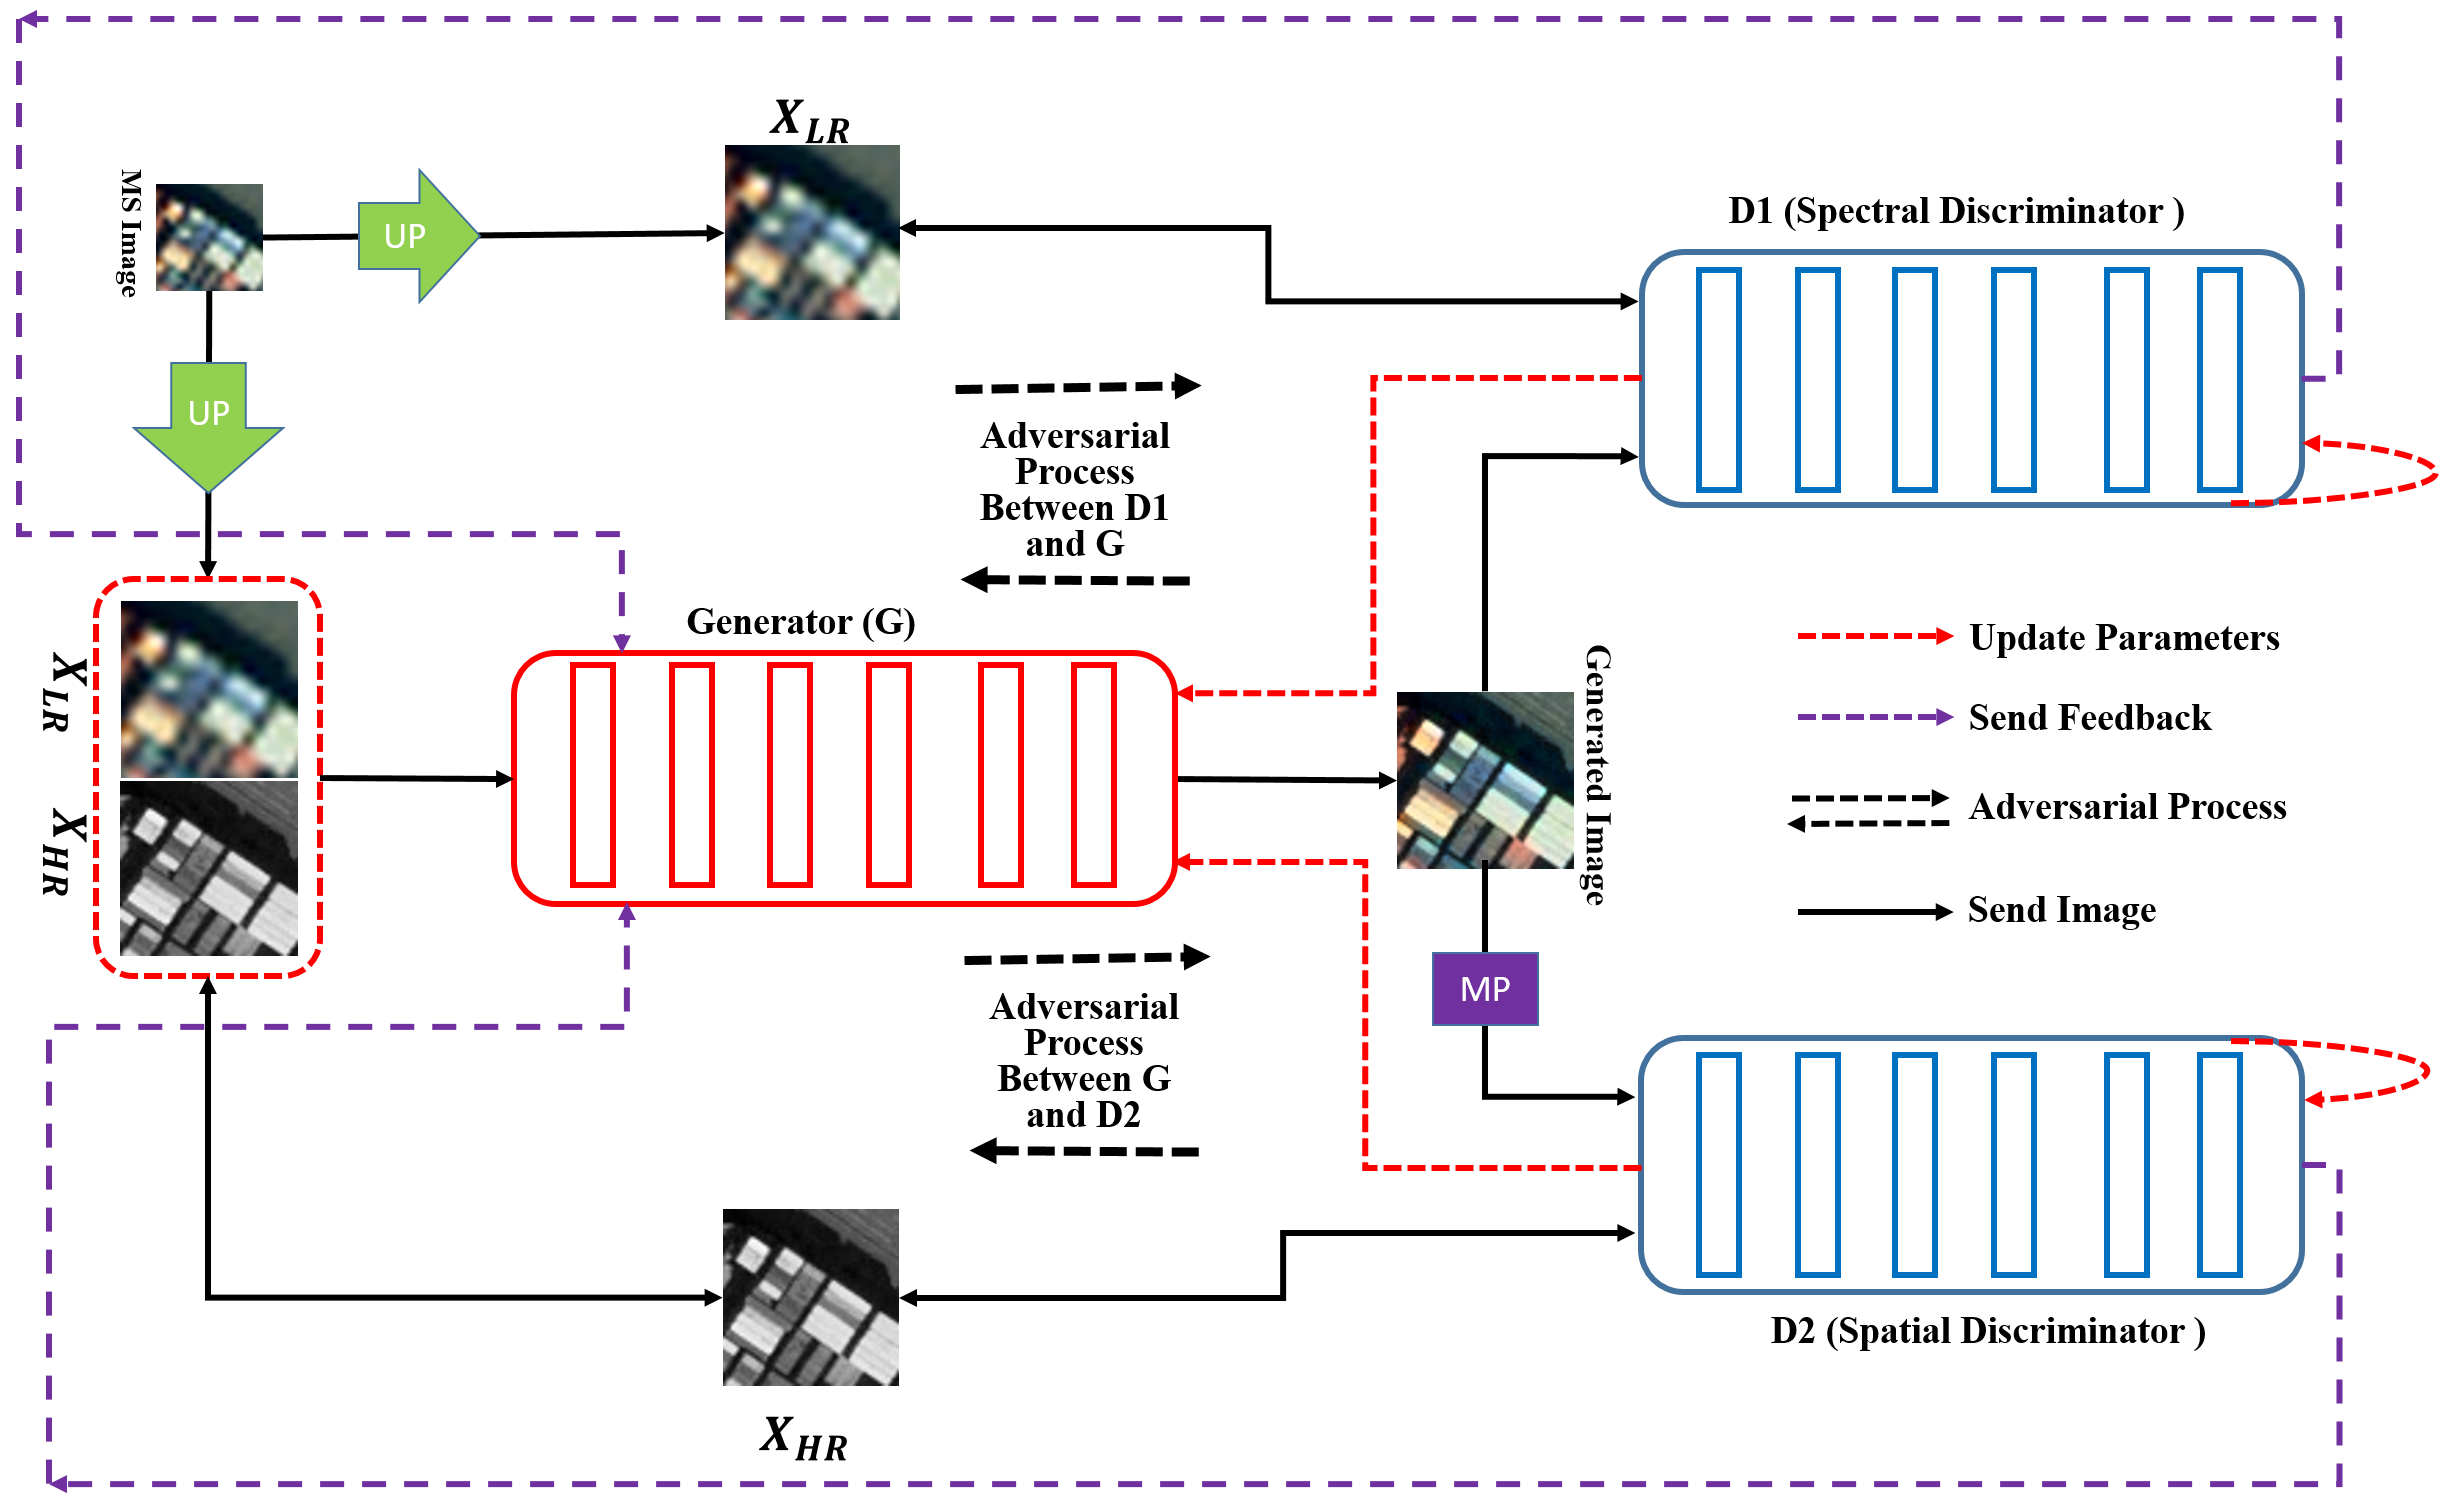
\includegraphics[width=1.0\linewidth]{GAN_ARCH}
\caption{Remote Sensing System}
\label{Fig:f1}
\end{center}
\end{figure}

\section{System Architecture}  
\section{Data Flow Diagrams}  
	
\section{Entity Relationship Diagrams)}   
\section{UML Diagrams} 

\chapter{Software Implementation}
\section{Technology Details used in the Project}
\section{Dataset Used in the Project}

\chapter{Project Estimation, Schedule and Team Structure}
\section{Project Cost}
Use of COCOMO model or any other relevant model for cost estimation
\section{Project Schedule and Team Structure}
For project schedule you may use time line chart.

\chapter{Software Testing and Validation}
\section{Type of Testing}
\section{Test Case}
\section{Risk Management}
Risk Identification and Risk Analysis

\chapter{Result and Analysis}
Description about Dataset Used.
Implementation Details.
Metrics used for Evaluation e.g. confusion metrics, Sensitivity, Recall, Precision etc. (May change accordingly to project)
Qualitative (Visual results e.g. Input and Output images) and Quantitative (Tables or Graphs) Analysis

\chapter{Advantages, Limitations and Application}
\section{Advantages}
\section{Limitation}
\section{Applications}


\chapter*{Summary and Conclusion}
\addcontentsline{toc}{chapter}{Summary and Conclusion}
Write one page summary and conclusion 
May include separate paragraph for Future Work or Extension of Project by other Students


\bibliographystyle{unsrt}
\bibliography{RishikeshTambe}

\begin{appendices}
% \chapter{ALGORITHMIC DESIGN}
\chapter{Awards/Participation in Project Competition/Exhibition}
\begin{itemize}
\item Problem statement feasibility assessment using, satisfiability analysis and NP Hard,NP-Complete or P type using modern algebra and relevant mathematical models.\\ 
\end{itemize}

\chapter{Details of the Papers Publication (if any)}
Details of the papers referred in IEEE format (given earlier) Summary of the above paper in not more than 3-4 lines. Here you should write the seed idea of the papers you had referred for preparation of this project  report in the following format.
\newline
Example: 
Thomas Noltey, Hans Hanssony, Lucia Lo Belloz,”Communication Buses for Automotive Applications” In Proceedings of the 3rd Information Survivability Workshop (ISW-2007), Boston, Massachusetts, USA, October 2007. IEEE Computer Society.

\chapter{Plagiarism Report For this Report}
All must attach certificate/report of Plagiarism issued by Urkund Software. Percentage of Similarity should not be more than 30\%  

\chapter{Any other Documentation evidences related to Project}
All must attach certificate/report of Plagiarism issued by Urkund Software. Percentage of Similarity should not be more than 30\%  

\end{appendices}


\end{document}
